\section{Contribution}\label{sec:cont}
The specific problem tackled by this research is: ``\textit{is it possible to automatically identify exploitable SQL injections flaws on PHP code without execute it?}''. 

Code \ref{cod:vuln01} presents a simplest example of vulnerable code which we expect to uncover. A string is received through HTTP POST method and used for composing the query without any sanitisation. 

\begin{lstlisting}[caption=Example of simplest vulnerable code,label=cod:vuln01]
<?php
$id = $_POST['id'];
$query = "SELECT name, email from users where id = ". $id;
$result = pg_query($conn, $query);
?>
\end{lstlisting}

Another situation very common and less trivial to detect by a manual approach is when the query is distributed among different functions as showed in Code \ref{cod:vuln02}. This is an illustration example, but between the function call and the use of the string inside the query can have a huge number of manipulations. For instance the example showed on Code \ref{cod:vuln02} has a vulnerability on line $3$ once the user can manipulate cookie values. The proposed approach also aims to automatically detect such kind of scenario.

\begin{lstlisting}[caption=Example of vulnerable code with multiple functions,label=cod:vuln02]
<?php
function get_limits() {
	$page_size = $_COOKIE['page_size']
	$index = $_COOKIE['page_size'] * (int) $_POST['page'];
	return "limit $index, $page_size;"  
}

function get_user_fields() {
	return " name, email "
}
$query = "SELECT ". get_user_fields() ." from users". get_limits();
$result = pg_query($conn, $query);
?>
\end{lstlisting}

Aiming detecting such kind of vulnerabilities the proposed method was divided in $4$ steps \footnote{in despite of using PHP code as analysed technology, this method can be applied to any other programming language which interacts with a database}:

\begin{itemize}
	\item Input patterns: conventions details about input variables must be provided according to the analysed technology;
	\item pre-processing: exclude comments, isolates the code that will be analysed, detect variables and try to determine their types by observing assignment statements;
	\item Pattern matching: enumerate all string variables and try to find SQL patterns, enumerate SQL strings concatenations \footnote{the concatenation syntax for the analysed language has to be formally described};
	\item Taint analysis: perform a backward taint analysis from the found variables inside concatenated SQL strings;
	\item Output: alert for variables used for assembly SQL queries which have some influence from input variables.
\end{itemize}  

\subsection{Input Pattern Step}

The Input Pattern step aims to define input patterns according to the analysed technology. As we state before, for analysing the source code using a static approach which doesn't have access to runtime information, we have to provide some heuristic or information about input variables labels. Table \ref{tab:input_variable_labels} presents a list of possible input variable labels for PHP language. All PHP code presented in this session will be analysed through \textit{Ruby} scripts.

\begin{table}[ht] 
\caption{Input Variables for PHP Language}
\centering
\begin{tabular}{c c}
\hline\hline
Label & Description \\ [0.5ex]
\hline
\$\_SERVER & Contains headers, paths, and script locations \\
\$\_GET & Items uploaded via the HTTP GET method\\
\$\_POST & Items uploaded via the HTTP POST method\\
\$\_FILES & Items uploaded via the HTTP POST method\\
\$\_REQUEST & Contents of \$\_GET, \$\_POST and \$\_COOKIE\\
\$\_SESSION & Array containing session variables\\
\$\_ENV &  Variables passed via the system environment\\
\$\_COOKIE & Array of variables passed via HTTP Cookies\\
\$argc & Number of arguments (command line)\\
\$argv & Arguments (command line)\\

\hline
\label{tab:input_variable_labels}
\end{tabular}
\end{table}

The algorithm should seek by these patterns inside the output of the Backward Taint Analysis step to see if variables used for composing the SQL string receive some influence from input variables controlled by an external user. As you can see this step works as a parameter for the proposed method and changes according the analysed technology. Each technology or framework has it own set of input variable.    

\subsection{Pre-Processing Step}
The pre-processing step is the first one that can be completely automated. This step aims clean the code and collect information about used variables along the source code. For this step we need to do a little \textit{compilers} work. First of all we have to describe the syntax of assignment statements and code comments for the analysed technology. For illustrating we describe these characteristics for PHP Language.

first of all we should treat the code for separate PHP code from HTML/Javascript/CSS code \footnote{This is a bad practice but most of PHP systems mix formatting code with the main code}. For performing this task we formally describe the convention for specifying code on PHP scripts through an finite automata. Figure \ref{fig:php_code_automata} show us the suggest automata for detect PHP code between tags ``$<?php$'' and ``$?>$'' or ``$<?$'' and ``$?>$''.

\begin{figure}[ht]
\centering
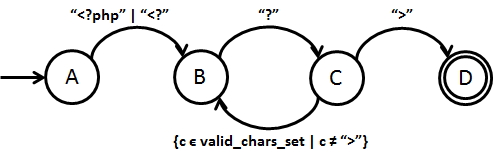
\includegraphics[width=0.75\textwidth]{image/automata.png}
\caption{Finite Automata for detecting PHP code pattern}
\label{fig:php_code_automata}
\end{figure}

This the specific syntax for code written in PHP for WEB applications under ``\textit{mod\_php}'', stand alone PHP code does not need this step once  ``.php'' files do not contain client-side and format code (\textit{e.g.} HTML, Javascript and CSS). 

Then, We should describe formally the syntax for code comments in PHP language. According its specification comments can be elaborated by three different ways. Code \ref{cod:php_comment} show us all possibilities for comments in PHP.

\begin{lstlisting}[caption=PHP code comments,label=cod:php_comment]
// one line comment
# one line comment
/* multi line comments */
\end{lstlisting} 

Once we only need remove those comments, we can easily describe those structures by using regular expressions. Code \ref{cod:php_comment_re_output} on lines 8, 11 and 14 show us example of regular expressions in Ruby that match with each PHP comment style.

\begin{lstlisting}[caption=Regular expressions for each code comment structure in PHP, label=cod:php_comment_re_output]
1.9.3-p194 :045 > print code
$var_01 = "marcos alvares" // one line comment;
# one line comment 02
/*
multi line comments
*/

1.9.3-p194 :046 > code =~ /(\/\/.*$)/; $1
 => "// one line comment;"

1.9.3-p194 :048 > code =~ /(#.*$)/; $1
 => "# one line comment 02"

1.9.3-p194 :050 > code =~ /(\/\*(.|\n)*\*\/)/; $1
 => "/*\nmulti line comments\n*/"
\end{lstlisting}

Then we have to extract information about label, position and type of variables along the code. PHP is a object oriented language then we have to describe the structure of classes, methods, standalone functions and assignment statements. We will store information about ``\textit{file name}'', ``\textit{class name}'', ``\textit{method name}'', ``\textit{label}'', ``\textit{type}'' and ``\textit{line number}'' for each variable founded inside the code. For variables inside the global scope the ``\textit{class}'' and ``\textit{method}'' name will be ``\textit{global}''. For variables inside standalone functions we will use ``\textit{global}'' for ``\textit{class name}''. Code \ref{cod:php_main_structures} show us these main structures that we are interested in detect and extract information about assign statements.

\begin{lstlisting}[caption=Three different scenarios of assignment statements in PHP code, label=cod:php_main_structures]
class Test {
    function method_01() {
        $var_01 = 'marcos';
    }
}

function function_01(){
	$var_01 = 'alvares';
}

$var_01 = 'marcos alvares';
\end{lstlisting}

From Code \ref{cod:php_main_structures} our algorithm should assembly a knowledge base containing information similar to Table \ref{tab:variables_table}. This information will be used for tracking all changes in variables along the source code and for performing the taint analysis.

\begin{table}[ht] 
\caption{Variables Information Table}
\centering
\begin{tabular}{c c c c c}
\hline\hline
label & class & method & line & file \\ [0.5ex]
\hline
\$var\_01 & Test & method\_01 & 3 & main.php \\
\$var\_01 & global & function\_01 & 8 & main.php \\
\$var\_01 & global & global & 11 & main.php \\
\hline
\label{tab:variables_table}
\end{tabular}
\end{table}

Until now we already have cleaned the code removing all format code and comments, now we should extract information about variables used within the analysed code and assembly the Table \ref{tab:variables_table}. For achieve this information, we should formally describe the above mentioned structures for PHP language by using syntax analysis techniques. Aiming produce a simplified parse for accomplishing our purpose of collect assignment statements, we described main structures of PHP by using the follow abstract syntax:

\begin{eqnarray*}
S & ::= & S;\:S \\
S & ::= & Com\:|\:Exp\:|\:Dec \\
S & ::= & \emptyset \\
SO & ::= & SO;\:SO \\
SO & ::= & Com\:|\:Exp\:|\:Dec\:|\:ProcDec\:|\:ObjDec \\
SO & ::= & \emptyset \\
ObjDec & ::= & class\:ClassName\:\{\:Dec\:|\:ProcDec\:\}; \\
ProcDec & ::= & function\:ProcName(Params)\:\{S\} \\
Dec & ::= & \$VarName = Exp\:|\:Value\:|\:Func \\
Dec & ::= & \$VarName = ClassName.new(Params) \\
Params & ::= & VarName\:|\:Func \\
Params & ::= & VarName,\:Params \\
DecParams & ::= & VarName\:|\:Value \\
DecParams & ::= & DecParams,\:DecParams \\
Value & ::= & Num\:|\:String\:|\:Bool \\
Exp & ::= & var\:op\:Exp \\
Exp & ::= & Com|Value \\
Com & ::= & if(Exp)\:\{\:S\:\}\:else\:\{\:S\:\} \\
Com & ::= & for(Dec;Exp;Exp)\:\{\:S\:\} \\
Com & ::= & while(Exp)\:\{\:S\:\} \\
Com & ::= & require(Exp) \\
\end{eqnarray*}

This is a very simplified description for the syntax of PHP Programming language, for instance, all functional structures, complex structs and specific commands were intentionally omitted. 

Finally the last activity related with pre-processing step is extract information about connections among PHP files. PHP uses the directive ``\textit{require()}'' for loading modules. This information can be obtained through the parser generated from the our abstract syntax once ``require'' is a command of PHP language. Table \ref{tab:kb_require} show us an hypothetic  example of which information we need to extract. For instance the first line means that ``\textit{module\_01.php}'' have a ``\textit{require()}'' statement to ``\textit{module\_02.php}'' on line $4$. From this data we can build a  graph with the information about who is connected with who where the modules are nodes and each line is an edge.

\begin{table}[ht] 
\caption{Modules Connections Table}
\centering
\begin{tabular}{c c c}
\hline\hline
from & to & line \\ [0.5ex]
\hline
module\_01.php & module\_02.php & $4$ \\
module\_01.php & module\_03.php & $31$ \\
module\_02.php & module\_03.php & $3$ \\
module\_03.php & module\_04.php & $2$ \\
\hline
\label{tab:kb_require}
\end{tabular}
\end{table}

\subsection{Pattern Matching Step}
At this point we already have information about all variables and assignment statements over the analysed code. Instead to be concerned with all tracks of all variables, we are concerned only with ``\textit{String}'' variables that contains patterns of \textit{SQL} once we are trying to identify possible failures on data input validation that are used for compose those queries. 

For Performing this task we have to extend our abstract syntax to describe ``\textit{String}'' patterns and some ``\textit{String}'' manipulation functions. ``ValidChar'' is any valid \textit{UTF-8} character different than ``\textbackslash0''.

\begin{eqnarray*}
Func & ::= & sprintf(String,\:params) \\
Func & ::= & vprintf(String,\:\$VarName) \\
Func & ::= & vsprintf(String,\:\$VarName) \\
String & ::= & ``chars'' \\
String & ::= & `chars' \\
Chars & ::= & ValidChar\:\&\:Chars \\
Chars & ::= & ValidChar \\
Chars & ::= & \symbol{92}0 \\
op & ::= & .|+|-|/ \\
\end{eqnarray*}

Table \ref{tab:sql_patterns} presents some SQL patterns\footnote{Some of those structures are specific of MySQL databases since this is the most used database on Wordpress CMS (related with our experiments) based systems} to be matched inside those detected \textit{Strings}. Its recommended also some \textit{ranking} heuristic for reduce the number of false positives. A reasonable heuristic is count how many keywords was found inside the string and define a threshold, for instance: only strings which has more than three SQL matches will be analysed.   

Note that concatenation operations is covered by our formal description once ``\textit{Exp}'' can be a ``\textit{Value}'' and the ``\textit{Value}'' can be a ``\textit{String}''. We also present the formal description for internal PHP API that also make concatenation operations like: ``\textit{sprintf()}'', ``\textit{vprintf()}'' and ``\textit{vsprintf()}''.

\begin{table}[ht] 
\caption{SQL Patterns}
\centering
\begin{tabular}{c c c c c}
\hline\hline
select & insert & update & delete & alter \\
from & union & where & order & limit \\
group & into & values & like & substr \\
trim & concat & timestamp & curdate & date\_format \\
unix\_timestamp & md5 & encrypt & sha1 & table \\
round & is\_empty & rand & count & not in \\
\hline
\label{tab:sql_patterns}
\end{tabular}
\end{table}

Then this step returns a list of \textit{``String''} concatenations statements  which contains such SQL patterns and at least one of the parameters of the concatenation operation is a variable. Code \ref{cod:concat_pattern} presents an example of such kind of pattern we are looking for. Note that our abstract syntax also cover ``\textit{String}'' interpolation.

\begin{lstlisting}[caption=String concatenation statement pattern, label=cod:concat_pattern]
if ( !empty( $profile_group_id ) )
  $where_sql = $db->prepare('WHERE g.id = %d', $profile_group_id);
elseif ( $exclude_groups )
  $where_sql = "WHERE g.id NOT IN ({$exclude_groups})";
\end{lstlisting}

The string listed on line $4$ should be classified as suspicious and the variable ``\textit{\$exclude\_groups}'' should be analysed to see if receives some influence from input parameters showed on Table \ref{tab:input_variable_labels}.

\subsection{Taint Analysis Step}

At this point we have information about all variables and found patterns of specific strings concatenation statements. Now we should extract the backward track of tainted variables from the detected variable within the concatenation statement. If the tainted set has any variable listed on the user input variable set the algorithm will warn about a potential SQL Injection failure.

Algorithm \ref{alg:taint} show us a pseudo-code for performing a backward taint analysis of variables extracted during the above mentioned steps. This code is supposed to receive a set of vulnerabilities and return a set of taint analyses for each provided variable. 

This step is also responsible for verifying the presence of user input variables on each returned analysis once we are only interested on ones that contains user input variables. This can represent an Valid SQL Injection attack once the user can manipulate queries used through the application.

Next session we show the application of these steps for uncover SQL Injections vulnerabilities on a popular Content Management System written in PHP called Wordpress. This application is expansible and have powerful plugin engine. We applied the proposed method for testing approximately $23.000$ Wordpress plugins downloaded from the Official website \footnote{http://wordpress.org/extend/plugins/}.

\begin{algorithm}
\caption{backward taint analysis algorithm}
\label{alg:taint}

\begin{algorithmic}
\STATE Initialise a pool of variables to be analysed (1)
\STATE Initialise an output pool for store taint analysis for all analysed variables (2)

\REPEAT
  \STATE Set the current analysed variable to the top of the pool of variables to be analysed (1)
  \STATE Exclude variable located on top of the pool of variables to be analysed (1)
  \STATE Initialise a pool (3) which represents the tainted variables for the current analysed variable
  \REPEAT
    \STATE Get information about type and scope of the analysed variable
    \STATE Follow the flow backward until find a taint point
    \IF{find some taint point}
      \STATE Store the current analysed variable on top of tainted vector (3)
      \STATE Set the current analysed variable as the tainted variable
    \ENDIF
  \UNTIL{No more taint point}
  \STATE Store the pool (3) inside the output pool (2)
\UNTIL{All variables are analysed}

\STATE return an output pool with taint analysis for all analysed variables (2) 
\end{algorithmic}
\end{algorithm}


